\subsection{Examples}

We now present some examples where we use Theorem \ref{thm_positive_rank} to force positive rank. Throughout we will consider an elliptic curve $E$ defined over $\bQ$, and a finite Galois extension $F / \bQ$ with Galois group $G = \Gal(F / \bQ)$. We let $\Delta_E$ denote the global minimal differential of $E / \bQ$. 
%As described in Remark \ref{rephrase-thm}, the strategy is to find a representation $\rho$ of $G$ and a $\rho$-relation $\Theta \in \B(G)$ such that $C(\Theta)$ is either not a norm from a quadratic subfield of $\bQ(\rho)$, or not a rational square, as appropriate. 
We start with a small observation:

\begin{rem}[Taking quotients]
   Let $E$, $F$, $G$ be as above. Consider $H \leq G$, and $N \triangleleft G$ such that $N \leq H$. Let $L = F^N$. Then $C_{E / F^H}$ is equal to $C_{E / L^{H/N}}$ as the fields $F^H$ and $L^{H/ N}$ are isomorphic. 
    
%    Consider a representation $\rho$ of $G$ with $N \leq \ker \rho$, so that $\bQ(\rho) = \bQ(\rho^N)$. Then, if $\Theta = \sum_i n_i H_i \in \B(G)$ with $N \leq H_i$ for all $i$, it follows that $N \cdot \Theta / N = \Theta / N$ being a norm relation for $C \colon \B(G / N) \to \bQ^{\times}$ implies that $\Theta$ is a norm relation for $C \colon \B(G) \to \bQ^{\times}$. 
\end{rem}

%We will be computing the terms $C_{E / F^H}$ for $F_i \subset F$ locally. Thus given a prime $p$ and subfield $F_i = F^H$ for 


When computing Tamagawa numbers, we will need to be able to count primes and compute ramification degrees in intermediate extensions of $F / \bQ$, which is described by the following. 

\begin{exercise}[Counting primes and ramification degrees]\label{ex-counting}
Consider a prime $p \in \bQ$ and decomposition and inertia groups $D_p$, $I_p \leq G$. Let $H \leq G$. 
\begin{enumerate}
    \setlength\itemsep{0em}
    \item The number of primes above $p$ in $F^H$ is given by the number of orbits of $D_p$ on $H \backslash G$, where $D_p$ acts by $d(Hg) = H g d^{-1}$ for $d \in D_p$. Equivalently it is $|H \backslash G / D_p|$.
    \item Let a prime $\fP$ above $p$ in $F^H$ correspond to an orbit $Y$ of $D_p$ acting on $H \backslash G$. Then the inertia degree of $\fP$ over $\bQ$ is the size of the $I_p$ sub-orbits on $Y$. 
\end{enumerate}
\end{exercise}


\begin{example}[Brauer relation forces growth]\label{ex-C2C6}
    Let $G = C_2 \times C_6$, with subgroup diagram
    \begin{figure}[H]
        \centering
    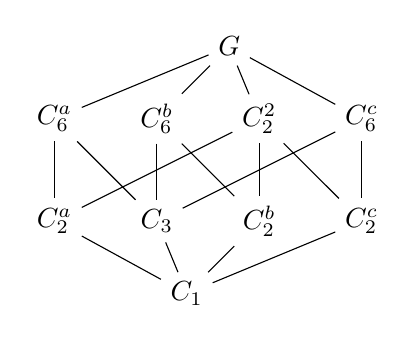
\begin{tikzpicture}[node distance=1.3cm]
        \node(G)[midway]{$G$};
        \node(C6b)[below left of =G]{$C_6^{b}$}; \node(C6a)[left of=C6b]{$C_6^{a}$};  
        \node(C22)[right of=C6b]{$C_2^{2}$};    \node(C6c)[right of=C22]{$C_6^{c}$};
        \node(C2a)[below of=C6a]{$C_2^{a}$};    \node(C3)[below of=C6b]{$C_3$};
        \node(C2b)[below of=C22]{$C_2^{b}$};    \node(C2c)[below of=C6c]{$C_2^{c}$};
        \node(C1)[below left of=C2b]{$C_1$};
        \draw(G)--(C6a);    \draw(G)--(C6b);    \draw(G)--(C6c);    \draw(G)--(C22);
        \draw(C6a)--(C2a);  \draw(C6a)--(C3);
        \draw(C6b)--(C2b);  \draw(C6b)--(C3);
        \draw(C6c)--(C2c);  \draw(C6c)--(C3);
        \draw(C22)--(C2a);  \draw(C22)--(C2b);  \draw(C22)--(C2c);
        \draw(C2a)--(C1);   \draw(C2b)--(C1);   \draw(C2c)--(C1);   \draw(C3)--(C1); 
    \end{tikzpicture}
    \end{figure}
    %There is a Brauer relation coming from the $C_2 \times C_2$-quotient, given by $$\Psi = C_3 - C_6^a - C_6^b - C_6^c + 2G.$$ 
    
    Consider an order $6$ character $\rho_a$ of $G$ with $C_2^{a}$ in its kernel. This has $\bQ(\rho_a) = \bQ(\zeta_6) = \bQ(\sqrt{-3})$. Let $\tau$ generate $\Gal(\bQ(\rho_a) / \bQ)$. One has
    \begin{equation}\label{ex1-rel}\tag{\textdagger}
    \Ind_{C_2^{a}}^G \trivial  \ominus \Ind_{C_6^{a}}^G \trivial \ominus \Ind_{C_2^{2}}^G \trivial \oplus \Ind_G^G \trivial \simeq \rho_a \oplus \rho_a^{\tau} .
    \end{equation}
    Let $E / \bQ$ be a semistable elliptic curve. To apply Theorem \ref{thm_positive_rank}, we need to compute
    \begin{equation}\label{ex1}\tag{*} 
        \frac{C_{E / F^{C_2^a}} C_{E / \bQ} }{C_{E / F^{C_6^a}} C_{E / F^{C_2^2}}} = 
        \frac{C_{E / L} C_{E / \bQ}}{C_{E / L^{C_3}} C_{E / L^{C_2}}}
    \end{equation} 
    where $L = F^{C_2^a}$ has $\Gal(L / \bQ) = C_6$, and check whether it is a norm from $\bQ(\sqrt{-3})$. This is a product of local Tamagawa numbers, as the minimal differential terms are $1$ when $E / \bQ$ is semistable (Lemma \ref{lem_Dterms}(i)). 
    
    One needs to compute these locally for each $p \in \bQ$. If $E / \bQ_p$ has good reduction, then the Tamagawa numbers at all places above $p$ in the subfields of $L$ are $1$. Suppose that $E / \bQ_p$ has split multiplicative reduction at $p$. Let $n = v_p(\Delta_E)$. For $H \leq G$, the Tamagawa number at a prime $\fP$ above $p$ in $L^H$ is given by $c_{\fp}(E / L^H) = e_{\fP \mid p} n$, where $e_{\fP \mid p}$ is the ramification degree. Thus the computation of Tamagawa numbers depends on the choice of decomposition group $D_p \leq C_6$ (to count the number of primes above $p$ in a given subfield) and the choice of inertia group $I_p \leq C_6$ (to compute the ramification indices). 
    
    The following table describes the product of Tamagawa numbers at places above $p$ in our expression, for varying $D_p$ and $I_p$. We let $T_{\fP \mid p}(E / L^H) = \prod_{\fP \mid p}c_{\fP}(E / L^H)$ for $H \leq \Gal(L / \bQ)$ as defined in Notation \ref{not_contr}. Let $C_p = c_p(E / \bQ)T_{\fP \mid p}(E / L) \big/ T_{\fP \mid p}(E / L^{C_3})T_{\fP \mid p}(E / L^{C_2})$. 
    \[
    \begin{array}{c c c c c c c}
        D_p & I_p & c_p(E / \bQ) & T_{\fP \mid p}(E / L^{C_3}) & T_{\fP \mid p}(E / L^{C_2}) & T_{\fP \mid p}(E / L) & C_p\\ 
        \hline
        C_1 & C_1 & n & n^2 & n^3 & n^6 & \square\\
        C_2 & C_1 & n & n & n^3 & n^3 & \square\\
        C_3 & C_1 & n & n^2 & n & n^2 & \square \\
        C_6 & C_1 & n & n & n & n & \square \\
        C_2 & C_2 & n & 2n & n^3 & (2n)^3 & \square \\
        C_6 & C_2 & n & 2n & n & 2n & \square \\
        C_3 & C_3 & n & n^2 & 3n & (3n)^2 & 3\cdot\square \\
        C_6 & C_3 & n & n & 3n & 3n & \square\\
        C_6 & C_6 & n & 2n & 3n & 6n & \square
    \end{array}
    \]

    In all cases we see that $C_p$, the contribution of Tamagawa numbers above $p$, is a norm form $\bQ(\sqrt{-3})$. It is not too hard to check that this is also the case when $E / \bQ_p$ has non-split multiplicative reduction. Therefore the expression in \eqref{ex1} is always a norm from $\bQ(\rho_a)$. This is an example of a more general phenomenon; for cyclic groups we always get a norm. This follows from  Theorem \ref{thm_consistent_cyclic}, which is proven in \S\ref{sec_cyclic}.
    %and $F / \bQ$ an abelian extension with $G = \Gal(F / \bQ)$. We claim that $C(\Theta) \in \fieldnorm{\rho_a}$, for all such $E$. Since each subgroup in $\Theta$ contains $C_2^{a}$, we have that $C(\Theta)$ equals $C(\Theta / C_2^{a})$ where $\Theta / C_2^{a} \in \B(G / C_2^{a}) = \B(C_6)$.  Now $\Theta / C_2^{a}$ is a $\chi_6$-relation, where $\chi_6 = \rho_a^{C_2^a}$ is a faithful order $6$ character of $C_6$, with $\bQ(\chi_6) = \bQ(\rho_a)$. But for cyclic groups we always get norm relations; by Theorem \ref{thm_consistent_cyclic}, $C(\Theta / C_2^{a}) \in \fieldnorm{\rho_a}$.

    But! Observe that{\footnote{this is called a Brauer relation, see Definition \ref{def-brauer}}} 
    \[ \Ind_{C_3}^G \trivial \ominus \Ind_{C_6^a}^G \trivial \ominus \Ind_{C_6^b}^G \trivial \ominus \Ind_{C_6^c}^G \trivial \oplus (\Ind_G^G \trivial)^{\oplus 2} = 0 \]
    as a virtual permutation representation. Append this to the left hand side of \eqref{ex1-rel}. Then Theorem \ref{thm_positive_rank} asks us to compute 
    \begin{equation}\label{ex1-rel2}\tag{**}
    \left(\frac{C_{E / F^{C_2^a}} C_{E / \bQ} }{C_{E / F^{C_6^a}} C_{E / F^{C_2^2}}}\right) \cdot \left( \frac{C_{E / F^{C_3}} C_{E / \bQ}^2}{C_{E / F^{C_6^a}}C_{E / F^{C_6^b}}  C_{E / F^{C_6^c}} } \right). 
    \end{equation}
    
    We can find instances where the second factor is not a norm from $\bQ(\sqrt{-3})$. Indeed suppose $E / \bQ$ has split multiplicative reduction at a prime $p$ with $D_p = G$, $I_p = C_6^b$. Let $v_p(\Delta_E) = n$. Then there is only one prime above $p$ in each subfield. Suppose $E$ has good reduction at all other primes (or multiplicative reduction at primes that are totally split in $F / \bQ$ would also be fine).
     Then our expression \eqref{ex1-rel2} is equal to
     \[ \frac{(6n)(n)}{(2n) (3n)} \cdot \frac{(2n)(n)^2}{(2n)(n)(2n)} \cdot \square = \frac{1}{2} \cdot \square, \] 
     which is not a norm from $\bQ(\sqrt{-3})$. Hence one must have $\rk E / F > 0$. 
\end{example}

\begin{example}[Dihedral]
    Let $q_1, q_2$ be odd primes. Consider $G = D_{2 q_1 q_2}$ the dihedral group of order $2 q_1 q_2$. 
    Let $\rho$, $\tau_1$, $\tau_2$ be two-dimensional irreducible representations of $G$ corresponding to rotating a $(q_1 q_2)$-gon by $2 \pi / q_1 q_2$, $2 \pi / q_1$, $2 \pi/ q_2$ respectively. These are all self-dual. The Galois conjugates of these representations, as well as the trivial $\trivial$ and sign $\epsilon$, yield all the irreducible representations of $G$. Let 
    \[  \sigma_{\rho} = \bigoplus_{ \fg \in \Gal(\bQ(\rho) / \bQ)} \rho^{\fg}, \qquad
        \sigma_1 = \bigoplus_{ \fg \in \Gal(\bQ(\tau_1) / \bQ)} \tau_1^{\fg}, \qquad
        \sigma_2 = \bigoplus_{ \fg \in \Gal(\bQ(\tau_2) / \bQ)} \tau_2^{\fg}. \]  
    Then $ \{ \trivial , \epsilon, \sigma_{\rho}, \sigma_1, \sigma_2 \}$ are a basis for the irreducible representations of $G$ over $\bQ$. 
    One has
\[
        \Ind_{C_2}^G \trivial \simeq \trivial \oplus \sigma_1 \oplus \sigma_2 \oplus \sigma_{\rho}, \quad
        \Ind_{D_{2 q_1}}^G \trivial \simeq \trivial \oplus \sigma_2, \quad
        \Ind_{D_{2 q_2}}^G \trivial \simeq \trivial \oplus \sigma_1,
\]
% There is an irreducible representation $\rho$ of $G$, obtained by inducing a linear order $q_1 q_2$ faithful representation from $C_{q_1 q_2}$. Thus $\rho$ is of degree $2$ and $\bQ(\rho) = \bQ(\zeta_{q_1 q_2})^{C_2}$. Then $\rho$ has $\frac{(q_1 - 1)(q_2 - 1)}{2}$ Galois conjugates, and so $\repnorm{\rho}$ is of dimension $2 \cdot \frac{(q_1 - 1)(q_2 - 1)}{2}$. 
and so 
\begin{equation*}
\Ind_{C_2}^G \trivial \ominus \Ind_{D_{2 q_1}}^G \trivial \ominus \Ind_{D_{2 q_2}}^G \trivial \oplus \Ind_{G}^G \trivial \simeq \bigoplus_{ \fg \in \Gal(\bQ(\rho) / \bQ)} \rho^{\fg}.
\end{equation*}

    Assume $E / \bQ$ is semistable. Suppose that $E / \bQ_p$ has split multiplicative reduction, with $n = v_p(\Delta_E)$. We compute Tamagawa numbers above $p$ as in the previous example, using the same notation. 
    Corollary \ref{cor-odd-decomp} implies that we always get a norm from the contribution above $p$ whenever the decomposition group is a group of odd-order. In fact we only get a non-square contribution when the decomposition group is $D_{2 q_1}$ or $D_{2 q_2}$ (and $I_p$ is non-trivial). 
     
    For example, let $p$ have decomposition group $D_{2 q_1}$ and inertia group $C_{q_1}$.
    This time, counting primes and computing ramification degrees is a little more awkward, we use Exercise \ref{ex-counting}.
        \begin{itemize}[--]
            \setlength\itemsep{0em}
            \item The action of $D_{2 q_1}$ on $C_2 \backslash G$ yields $1$ orbit of size $C_{q_1}$ (the orbit of the identity) and $\frac{q_2 - 1}{2}$ orbits of size $2q_1$ (coming from $C_2$ acting faithfully on $C_{q_2}$). The size of the inertia sub-orbits is $q_1$. Hence $T_{\fP \mid p}(E / F^{C_2}) = (q_1 n)^{1 + \frac{q_2 - 1}{2}}$.
            
            \item The action of $D_{2 q_1}$ on $D_{2 q_1} \backslash G$ yields the same number of orbits as above, but now the action of $C_{q_1} \leq D_{2 q_1}$ is trivial, so that $T_{\fP \mid p}(E / F^{D_{2 q_1}}) = n^{1 + \frac{q_2 - 1}{2}}$.
            
            \item The action of $D_{2 q_1}$ on $D_{2 q_2} \backslash G$ yields one orbit of size $q_1$, with the inertia sub-orbit also of size $q_1$, hence $T_{\fP \mid p}(E / F^{D_{2 q_2}}) = q_1 n$.
        \end{itemize}
    In total,
    \[ \frac{T_{\fP \mid p}(E / F^C_2) \cdot c_{\fp}(E / \bQ)}{T_{\fP \mid p}(E / F^{D_{2 q_1}})\cdot T_{\fP \mid p}(E / F^{D_{2 q_2}})} = \frac{(q_1 n )^{1 + \frac{q_2 - 1}{2}} (n)}{(n)^{1 + \frac{q_2 - 1}{2}} (q_1 n)} = q_1^{\frac{q_2 - 1}{2}} .\] 
    %By symmetry, taking the decomposition group to be $D_{2 q_2}$ and inertia group $C_{q_2}$, one would obtain $ q_2^{\frac{q_1 - 1}{2}}$.

    So let $E / \bQ$ have split multiplicative reduction at $p$ with decomposition group $D_{2 q_1}$ and inertia group $I_p = C_{q_1}$, and good reduction at all other primes. Further suppose that $q_1, q_2 \equiv 3 \pmod 4$ and that $\legendre{q_1}{q_2} = -1$. Then $\bQ(\sqrt{q_1 q_2}) \subset \bQ(\rho)$ but 
$$\frac{C_{E / F^C_2} C_{E / \bQ}}{C_{E / F^{D_{2 q_1}}} C_{E / F^{D_{2 q_2}}}} = q_1 \cdot \square$$
is not a norm from $\bQ(\sqrt{q_1 q_2})$. Indeed, $q_1$ is not the norm of an element of $\bQ(\sqrt{q_1 q_2})$, since $z^2 q_1 = x^2 - q_1q_2 y^2$ for $x,y,z \in \bZ$ implies $q_1 = \square \pmod {q_2}$, a contradiction. Thus $\rk E / F > 0$.

    This rank growth is predicted by root number computations also, however. Assume that $F / \bQ$ is totally real. Then $w(E / F^H) = (-1)^{[F^H \colon \bQ] + | H \backslash G / D_p|}$ by Proposition \ref{compute-root}. Thus
    \begin{itemize}[--]
        \setlength\itemsep{0em}
        \item $w(E / \bQ) = (-1)^2 = 1$,
        \item $w(E / F^{C_2}) = (-1)^{q_1 q_2} (-1)^{1 + \frac{q_2 - 1}{2}} = (-1)^{\frac{q_2 - 1}{2}}$,
        \item $w(E / F^{D_{2 q_1}}) = (-1)^{q_2}(-1)^{1 + \frac{q_2 - 1}{2}} = (-1)^{\frac{q_2 - 1}{2}},$
        \item $w(E / F^{D_{2 q_2}}) = (-1)^{q_1}(-1) = 1$. 
    \end{itemize}
    Therefore we must have $\rk E / F^{C_2}$, $\rk E / F^{D_{2q_1}} > 0$, so $\rk E / F > 0$. 
    Using the properties in Proposition \ref{compute-root-twist}, the computations of the root numbers for the subfields implies that 
    \[ w\left(E / \bQ, \sigma_1\right) = 1, \quad w\left(E / \bQ, \sigma_2\right) = -1, \quad w\left(E / \bQ, \sigma_{\rho}\right) = 1, \]
  and in particular $w(E / \bQ, \tau_1^{\fg}) = -1$ for some $\fg \in \Gal(\bQ(\tau_1) / \bQ)$.
\end{example}

\begin{example}[Additive reduction example]
Let $G = C_{65} \ltimes C_4$, where $C_4$ acts faithfully on $C_{65}$, as well as the subgroups $C_{13}$ and $C_5$. By inducing a faithful character of order $65$ from $C_{65}$, one obtains a faithful irreducible representation $\rho$ of $G$ of dimension $4$ and with $\bQ(\rho) = \bQ(\zeta_{65})^{C_4}$. In particular one has $\bQ(\sqrt{65}) \subset \bQ(\rho)$. Then
\[ \Ind_{C_4}^G \trivial \ominus \Ind_{C_{13} \ltimes C_4}^G \trivial \ominus \Ind_{C_5 \ltimes C_4}^G \trivial \oplus \Ind_{G}^G \trivial \simeq \bigoplus_{\fg \in \Gal(\bQ(\rho) / \bQ)} \rho^{\fg} .\]
Therefore by Theorem \ref{thm_positive_rank}, either 
\begin{equation}\label{ex3}\tag{\textdagger \textdagger}
\frac{C_{E / F^{C_4}} C_{E / \bQ} }{C_{E / F^{C_{13} \ltimes C_4}} C_{E / F^{C_5 \ltimes C_4}}}
\end{equation}
is a norm from $\bQ(\sqrt{65})$, or $\rk E / F > 0$.  

Suppose $p = 5$ and $E / \bQ_p$ has additive, potentially good reduction. Further suppose that $F / \bQ$ is an extension such that $D_{5} = I_{5} = C_5 \ltimes C_4$ (this is wildly ramified). Let $n = v_p(\Delta_E) < 12$. Then
\begin{itemize}[--]
    \setlength\itemsep{0em}
    \item In $F^{C_4}$ there is one prime above $p$ with ramification degree $5$ and $3$ primes above $p$ with ramification degree $20$,
    \item In $F^{C_{13} \ltimes C_4}$ there is one prime above $p$ with ramification degree degree $5$,
    \item In $F^{C_5 \ltimes C_4}$ there is one prime above $p$ with ramification degree $1$ and $3$ primes above $p$ with ramification degree $4$.
\end{itemize}
Therefore, by Lemma \ref{lem_Dterms}(iii), the product of the minimal differential term is 
\[ \frac{D_{\fP \mid p}(E / F^{C_4}) D_{\fP \mid p}(E / \bQ) }{D_{\fP \mid p}(E / F^{C_{13} \ltimes C_4}) D_{\fP \mid p}(E / F^{C_{5} \ltimes C_4})} = 
\frac{ 5^{\floor{5 n /12}} \cdot \left(5^{\floor{20 n /12}}\right)^3 }{5^{\floor{5 n /12}} \left(5^{\floor{4 n /12}}\right)^3} .\]
If $n = 2$, then this is equal to $5 \mod {(\bQ^{\times})^2}$. By Lemma \ref{tamagawa-num} the Tamagawa number product is
\[ \frac{T_{\fP \mid p}(E / F^{C_4}) T_{\fP \mid p}(E / \bQ) }{T_{\fP \mid p}(E / F^{C_{13} \ltimes C_4}) T_{\fP \mid p}(E / F^{C_{5} \ltimes C_4})} = \frac{1^2 \cdot 3^3 }{1^2 \cdot 3^3} = 1 \text{ or } \frac{1^5}{1^5} = 1.\]

We claim that $5$ is not a norm from $\bQ(\sqrt{65})$. Indeed, $5z^2 = x^2 - 65 y^2$ for $x, y, z \in \bZ$ implies that $5 = \square \pmod 13$, a contradiction since $\legendre{5}{13} = \legendre{13}{5} = \legendre{3}{5} = -1$. Therefore the local contribution of \eqref{ex3} above $5$ is not a norm from $\bQ(\sqrt{65})$. 

What are the local root numbers above $p$? By Proposition \ref{compute-root}, one has
\begin{itemize}[--]
    \setlength\itemsep{0em}
    \item $w(E / \bQ_5) = (-1)^{\floor{ 10 / 12}} = 1$, 
    \item $\prod_{\fp \mid p} w(E /F^{C_4}_{\fp}) = (-1)^{\floor{50 / 12}} \left((-1)^{\floor{200 / 12}}\right)^3 = 1$,
    \item $\prod_{\fp \mid p} w(E /F^{C_{13} \times C_4}_{\fp}) = (-1)^{\floor{50 / 12}} = 1$,
    \item $\prod_{\fp \mid p}w(E /F^{C_{5} \times C_4}_{\fp}) = (-1)^{\floor{ 10/12}}\left((-1)^{\floor{40 / 12}}\right)^3 = -1$ .
\end{itemize}
Hence we see a change in the contributions of local root numbers above $p$ in the intermediate subfields. 




\end{example}